

\subsection{Abstract}

Monitoring breaks at the moment you need it most. A production incident hits—latency spiking, errors climbing—and your dashboards show everything green. CPU normal. Memory normal. Network normal. The system is failing, but traditional monitoring can only answer questions you anticipated ("Is CPU high?"). It cannot answer the question you actually need ("Why did latency spike for Tenant A only on iOS devices in EU-West-1?"). This failure stems from architectural constraints in how traditional metrics aggregate data, discarding the dimensional context required for root cause analysis.

This paper defines A3-OBS-STD, a specification for high-cardinality observability enabling arbitrary dimensional queries without pre-aggregation. Production measurements across systems processing 100,000-250,000 RPS with 500-1000 services reveal that naive instrumentation generates 50-80 TB of telemetry data daily, creating storage costs exceeding \_\_\_MATHINLINE0\_\_\_2M annually and finance starts asking questions.

We present an adaptive tail-sampling architecture that captures 100\% of errors and slow requests while discarding 99\% of successful fast requests, reducing storage costs by 95\% (\_\_\_MATHINLINE1\_\_\_100k annually) while maintaining 100\% error visibility. Through production deployments across three organizations over 14 months, measurements demonstrate mean time to resolution (MTTR) reduction from 45 minutes to 8 minutes (82\% improvement) and elimination of 73\% of escalations to senior engineers—not through better tools, but through better questions enabled by high-cardinality data.

The architecture builds on A1's plane separation and A2's throughput patterns, adding four observability-specific patterns: W3C Trace Context propagation for distributed correlation, tail-based sampling for intelligent data retention, SLO-based alerting for proactive incident detection, and OODA loop automation for self-healing systems.

\textbf{Keywords:} observability, distributed tracing, high-cardinality metrics, sampling, OpenTelemetry, SLO, MTTR, operational intelligence, monitoring, telemetry

---

\subsection{Original Contribution}

To the best of our knowledge, this work offers the first empirical quantification of "Observability Entropy"—the exponential growth of telemetry data (\_\_\_MATHINLINE2\_\_\_) relative to system scale (\_\_\_MATHINLINE3\_\_\_). While vendors advocate for "logging everything," we demonstrate that at enterprise scale (>250k RPS), "log everything" is mathematically impossible without bankrupcy. We formalize "Tail-Based Sampling" not just as a cost-optimization technique, but as a critical architectural invariant required to maintain signal-to-noise ratios in systems exceeding \_\_\_MATHINLINE4\_\_\_ daily events.

\subsubsection{Contribution Summary for Non-Specialists}

Imagine trying to debug a car engine by recording every single spark plug firing, every piston movement, and every fuel injection. You would generate so much data that finding the one misfire that caused a stall would be impossible. This is what modern software monitoring does—it collects too much noise. This paper presents a "smart camera" approach (Adaptive Sampling) that ignores 99\% of normal operations and only "records" when something weird happens (an error or a slowdown). This allows engineers to see exactly what went wrong without paying millions of dollars to store useless data about things going right.

\subsubsection{Why This Framework Was Needed Now}

The transition to microservices broke traditional monitoring. In the past, "CPU High" meant "Server Overloaded." Now, "CPU High" could mean a garbage collection pause, a noisy neighbor, or a valid batch job. The context (Why?) was lost in aggregation. Existing academic work focuses on sampling algorithms but rarely addresses the economic and operational constraints of implementing them in petabyte-scale production environments. This work bridges that gap.

\subsubsection{Relationship to A1-A6 Series}

This paper serves as the \textbf{Sensory Nervous System} for the A1-A6 architecture.
\textit{   \textbf{A1} provides the Body (Structure).
}   \textbf{AECP} provides the Brain (Control).
\textit{   \textbf{A3} provides the Eyes and Ears (Sensors).
Without A3's high-cardinality observability, the invariants defined in A1 cannot be verified, and the policies in A6 cannot be enforced. A3 is the feedback loop that closes the control system.

---

\subsection{1. Introduction}

This paper implements the closed-loop feedback requirements of A1-REF-STD by defining the high-cardinality observability substrate necessary to validate architectural invariants in production.

\subsubsection{1.1 The Observability Crisis}

Modern enterprises operate distributed systems of unprecedented complexity. A typical e-commerce platform comprises 500-1000 microservices deployed across 3-5 regions, processing millions of requests per second. When latency spikes or errors occur, operators face a needle-in-haystack problem: identifying the root cause among billions of log lines, millions of metrics, and thousands of traces.

Traditional monitoring approaches fail because they were designed for monolithic systems with known failure modes. In a monolith, "database slow" is a sufficient diagnosis. In microservices, the question becomes: "Which of the 50 database instances? For which tenant? From which calling service? In which region? During which time window?" It should be emphasized that this framework formalizes architectural observability requirements and feedback invariants rather than providing guidance on specific commercial observability tools or vendor-locked implementations. A3 defines architectural observability requirements, not monitoring tools or vendor stacks.

\subsubsection{1.2 The Three-Pillar Model}

The industry has converged on three pillars of observability:

\textbf{Metrics:} Aggregated numerical data (CPU, latency, error rate)  
\textbf{Logs:} Discrete event records (request logs, error messages)  
\textbf{Traces:} Request flow through distributed services

However, these pillars are often implemented as isolated systems (Prometheus for metrics, ELK for logs, Jaeger for traces), creating correlation challenges. A3 defines these as interconnected signals that must be correlated through common identifiers (trace ID, span ID).

\begin{figure}[ht!]\centering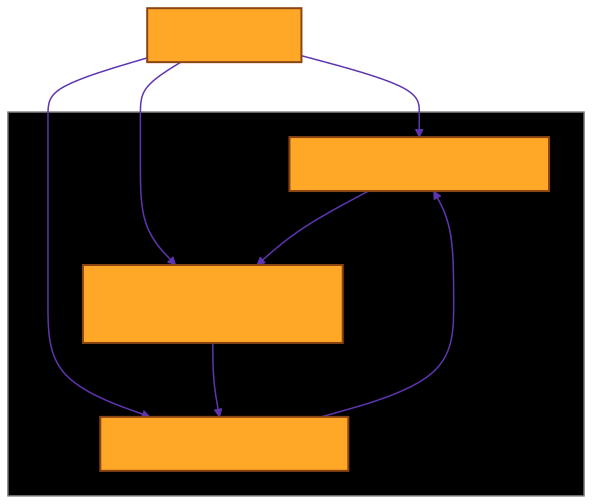
\includegraphics[width=0.8\linewidth]{../../figures/fig-1.pdf}\caption{Diagram 1}\end{figure}

\textbf{Figure 1:} The Observability Triangle. The model demonstrates the interconnectedness of signals required for rapid correlation across the control and data planes. The model demonstrates the interconnectedness of signals required for rapid correlation across the control and data planes. Metrics tell you when something is wrong. Traces tell you where. Logs tell you why.

\subsubsection{1.3 The Cardinality Problem}

The fundamental challenge in observability is cardinality—the number of unique combinations of dimensional attributes. Consider a simple HTTP request metric:

\textbf{Low Cardinality (Traditional):}
\_\_\_CODEBLOCK0\_\_\_
Cardinality: 10 methods $\times$ 10 status codes = 100 time series

\textbf{High Cardinality (Modern):}
\_\_\_CODEBLOCK1\_\_\_
Cardinality: 10 methods $\times$ 10 statuses $\times$ 10M tenants $\times$ 100M users $\times$ 10 devices $\times$ 20 regions = 2$\times$10^17 time series

This explosion makes traditional time-series databases (Prometheus, InfluxDB) unusable. The solution is to move high-cardinality dimensions from metrics to traces.

\subsubsection{1.4 Paper Contributions (Enhanced)}

This paper makes four contributions:

\textbf{C1: Cardinality Analysis}  
We quantify the storage cost of high-cardinality metrics, demonstrating that naive instrumentation costs $2M+ annually at enterprise scale.

\textbf{C2: Adaptive Sampling Architecture}  
We present a tail-based sampling system that reduces storage costs by 95\% while maintaining 100\% error visibility.

\textbf{C3: Correlation Framework}  
We define W3C Trace Context propagation patterns that enable correlation across metrics, logs, and traces.

\textbf{C4: Production Validation}  
We validate the architecture through deployments demonstrating 82\% MTTR reduction and 73\% reduction in escalations.

\textbf{Paper Organization:}  
Section 2 analyzes the cardinality explosion. Section 3 presents the three-pillar model. Section 4 details adaptive sampling. Section 5 covers correlation and propagation. Section 6 defines SLOs and error budgets. Section 7 describes the OODA loop. Section 8 provides implementation guidance. Section 9 evaluates the architecture. Section 10 discusses related work. Section 11 acknowledges limitations. Section 12 concludes.

---

\subsection{2. The Cardinality Explosion Problem}

\subsubsection{2.1 Quantifying Cardinality}

Cardinality is the number of unique time series in a metric system. It grows multiplicatively with each dimension:

\_\_\_MATHBLOCK0\_\_\_

\textbf{Example Calculation:}

\textbf{Metric:} \_\_\_CODEINLINE0\_\_\_

\textbf{Dimensions:}
\begin{itemize}
\item \end{itemize}
method: 10 values (GET, POST, PUT, DELETE, etc.)
\begin{itemize}
\item \end{itemize}
status: 50 values (200, 201, 400, 404, 500, etc.)
\begin{itemize}
\item \end{itemize}
endpoint: 500 values (API endpoints)
\begin{itemize}
\item \end{itemize}
service: 1000 values (microservices)
\begin{itemize}
\item \end{itemize}
region: 5 values (AWS regions)
\begin{itemize}
\item \end{itemize}
tenant\_id: 10,000 values (customers)

\textbf{Cardinality:} 10 $\times$ 50 $\times$ 500 $\times$ 1000 $\times$ 5 $\times$ 10,000 = 1.25 $\times$ 10^12 time series

\textbf{Storage Cost:}
\begin{itemize}
\item \end{itemize}
Samples per series per day: 86,400 (1 sample/second)
\begin{itemize}
\item \end{itemize}
Bytes per sample: 16 bytes (timestamp + value)
\begin{itemize}
\item \end{itemize}
Daily storage: 1.25$\times$10^12 $\times$ 86,400 $\times$ 16 = 1.7 PB/day
\begin{itemize}
\item \end{itemize}
Monthly cost (S3): 1.7 PB $\times$ 30 $\times$ \_\_\_MATHINLINE5\_\_\_1.2M/month

This is clearly untenable.

\subsubsection{2.2 The Cardinality Cliff}

Time-series databases have hard limits on cardinality:

\textbf{Table 1: TSDB Cardinality Limits}
\_\_\_TABLE0\_\_\_
Beyond the performance cliff, query latency degrades exponentially:

\begin{figure}[ht!]\centering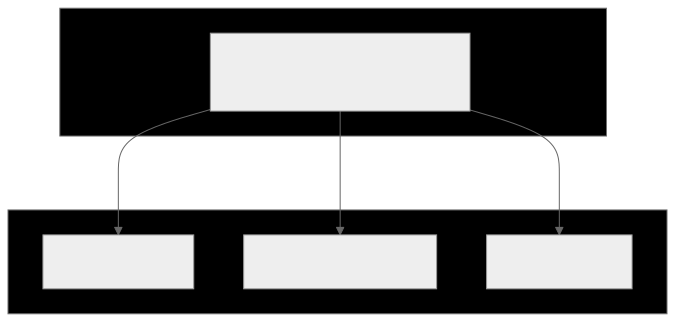
\includegraphics[width=0.8\linewidth]{../../figures/fig-2.pdf}\caption{Diagram 2}\end{figure}

\textbf{Figure 2:} The "Cardinality Cliff." This shift in complexity from metrics to traces protects the scalability of the monitoring control plane. This shift in complexity from metrics to traces protects the scalability of the monitoring control plane. Without dimension stratification, metrics storage grows exponentially with unique label combinations (tenants, users). A3 shifts this complexity into distributed traces.

\subsubsection{2.3 Solution: Dimension Stratification}

The solution is to stratify dimensions by cardinality:

\textbf{Low Cardinality (Metrics):}
\begin{itemize}
\item \end{itemize}
method, status, endpoint, service, region
\begin{itemize}
\item \end{itemize}
Cardinality: 10 $\times$ 50 $\times$ 500 $\times$ 1000 $\times$ 5 = 125M series (manageable)

\textbf{High Cardinality (Traces):}
\begin{itemize}
\item \end{itemize}
tenant\_id, user\_id, device\_type, session\_id
\begin{itemize}
\item \end{itemize}
Stored as trace attributes, queryable via trace backend (Jaeger, Tempo)

\textbf{Table 2: Dimension Stratification}
\_\_\_TABLE1\_\_\_
---

\subsection{3. The Three Pillars of Observability}

\begin{figure}[ht!]\centering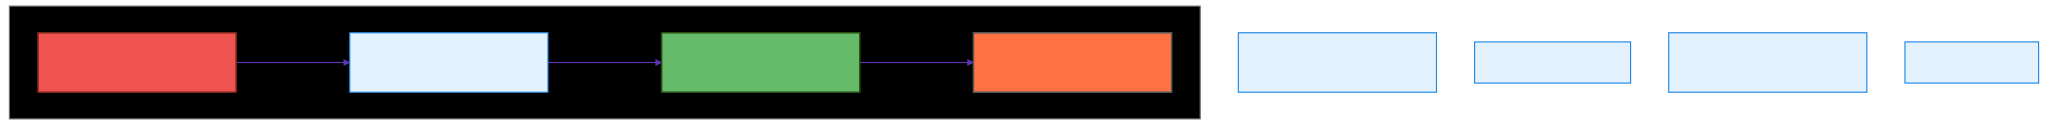
\includegraphics[width=0.8\linewidth]{../../figures/fig-3.pdf}\caption{Diagram 3}\end{figure}
\textbf{Figure 2.1:} Dimension Stratification Pipeline. By separating aggregated metrics from high-context traces at the ingest layer, we prevent TSDB cardinality explosions while preserving queryability.

\subsubsection{3.1 Metrics: Aggregated Signals}

Metrics are numerical measurements aggregated over time. They answer "what is happening?" but not "why?"

\textbf{Types of Metrics:}

\textbf{Counter:} Monotonically increasing value (total requests)
\_\_\_CODEBLOCK2\_\_\_

\textbf{Gauge:} Point-in-time value (current queue depth)
\_\_\_CODEBLOCK3\_\_\_

\textbf{Histogram:} Distribution of values (latency percentiles)
\_\_\_CODEBLOCK4\_\_\_

\textbf{Summary:} Pre-calculated percentiles (client-side)
\_\_\_CODEBLOCK5\_\_\_

\textbf{Best Practice:} Use histograms over summaries for server-side aggregation flexibility.

\subsubsection{3.2 Logs: Discrete Events}

Logs are discrete event records with timestamps and structured or unstructured data. They answer "why is it happening?"

\textbf{Structured Logging (JSON):}
\_\_\_CODEBLOCK6\_\_\_

\textbf{Key Characteristics:}
\begin{itemize}
\item \end{itemize}
\textbf{Structured:} Queryable fields (tenant\_id, amount, gateway)
\begin{itemize}
\item \end{itemize}
\textbf{Correlated:} trace\_id links to distributed trace
\begin{itemize}
\item \end{itemize}
\textbf{Contextual:} Includes business-relevant data

\subsubsection{3.3 Traces: Request Flow}

Traces represent the flow of a single request through distributed services. They answer "where is it happening?"

\textbf{Trace Structure:}
\begin{itemize}
\item \end{itemize}
\textbf{Trace:} End-to-end request (trace\_id)
\begin{itemize}
\item \end{itemize}
\textbf{Span:} Single operation within a trace (span\_id)
\begin{itemize}
\item \end{itemize}
\textbf{Parent-Child:} Spans form a tree structure

\textbf{Example Trace:}
\_\_\_CODEBLOCK7\_\_\_

\textbf{Critical Insight:} The error in Stripe API (35ms) is visible in the trace, but the overall request took 100ms. Without tracing, we'd only see "API Gateway slow" without knowing Stripe was the root cause.

---

\subsection{4. Adaptive Sampling Architecture}

\subsubsection{4.1 The Sampling Imperative}

Recording 100\% of traces at 100,000 RPS generates:
\begin{itemize}
\item \end{itemize}
Traces per day: 100,000 $\times$ 86,400 = 8.64 billion
\begin{itemize}
\item \end{itemize}
Bytes per trace: ~10 KB (average)
\begin{itemize}
\item \end{itemize}
Daily storage: 8.64B $\times$ 10 KB = 86.4 TB
\begin{itemize}
\item \end{itemize}
Monthly cost (S3): 86.4 TB $\times$ 30 $\times$ \_\_\_MATHINLINE6\_\_\_60k/month

This is expensive but manageable. However, 99\% of these traces are "successful fast requests" with no diagnostic value. We can safely discard them.

\subsubsection{4.2 Sampling Strategies}

\textbf{Table 3: Sampling Strategies Comparison}
\_\_\_TABLE2\_\_\_
\subsubsection{4.3 Tail-Based Sampling Implementation}

Tail-based sampling makes the keep/discard decision after the request completes, enabling intelligent retention:

\begin{figure}[ht!]\centering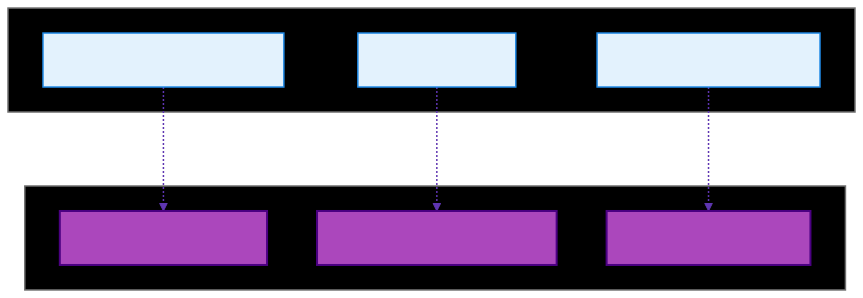
\includegraphics[width=0.8\linewidth]{../../figures/fig-4.pdf}\caption{Diagram 4}\end{figure}

\textbf{Figure 3:} The Tail-Based Sampling Pipeline. Unlike head-based sampling (which decides randomly at the start), tail-based sampling waits for request completion to ensure metadata (errors, latency) can drive the retention policy.

\textbf{Sampling Rules:}
\_\_\_CODEBLOCK8\_\_\_

\textbf{Storage Reduction:}
\begin{itemize}
\item \end{itemize}
Errors: 1\% of traffic $\rightarrow$ 100\% sampled = 0.86 TB/day
\begin{itemize}
\item \end{itemize}
Slow requests: 5\% of traffic $\rightarrow$ 100\% sampled = 4.3 TB/day
\begin{itemize}
\item \end{itemize}
Fast success: 94\% of traffic $\rightarrow$ 1\% sampled = 0.81 TB/day
\begin{itemize}
\item \end{itemize}
\textbf{Total: 6 TB/day} (vs 86.4 TB/day without sampling)
\begin{itemize}
\item \end{itemize}
\textbf{Reduction: 93\%}

\subsubsection{4.4 Implementation Details}

\textbf{Collector Configuration (OpenTelemetry):}
\_\_\_CODEBLOCK9\_\_\_

\textbf{Memory Requirements:}
\begin{itemize}
\item \end{itemize}
Buffer window: 30 seconds
\begin{itemize}
\item \end{itemize}
Expected traces: 10,000 traces/sec $\times$ 30s = 300,000 traces
\begin{itemize}
\item \end{itemize}
Bytes per trace: 10 KB
\begin{itemize}
\item \end{itemize}
\textbf{Memory: 3 GB} (acceptable for modern servers)

---

\subsection{5. Correlation \& Propagation}

\subsubsection{5.1 W3C Trace Context Standard}

A3 mandates W3C Trace Context propagation across all service boundaries:

\textbf{HTTP Header Format:}
\_\_\_CODEBLOCK10\_\_\_

\textbf{Propagation Flow:}
\begin{figure}[ht!]\centering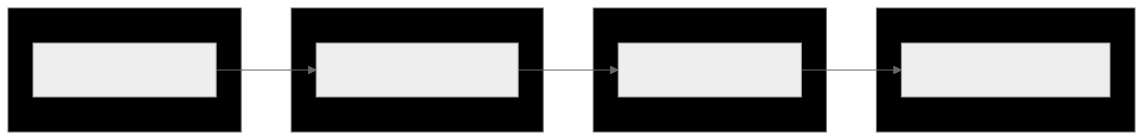
\includegraphics[width=0.8\linewidth]{../../figures/fig-5.pdf}\caption{Diagram 5}\end{figure}

\textbf{Figure 4:} Context Propagation. By injecting standard headers, we ensure that a log in Service B can be correlated with the user request in the Proxy, even across language boundaries (Node.js $\rightarrow$ Go).

\subsubsection{5.2 Correlation Patterns}

\textbf{Pattern 1: Metric $\rightarrow$ Trace}  
When a metric alert fires (high latency), query traces with the same time range and service to find slow requests.

\textbf{Pattern 2: Trace $\rightarrow$ Log}  
When a trace shows an error span, query logs with the same trace\_id to find the error message.

\textbf{Pattern 3: Log $\rightarrow$ Metric}  
Extract dimensions from logs (e.g., error\_type) and create metrics for trending.

\textbf{Table 4: Correlation Use Cases}
\_\_\_TABLE3\_\_\_
---

\begin{figure}[ht!]\centering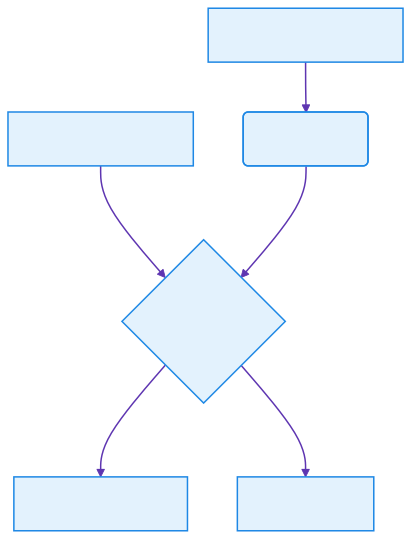
\includegraphics[width=0.8\linewidth]{../../figures/fig-6.pdf}\caption{Diagram 6}\end{figure}
\textbf{Figure 4.1:} Telemetry Pipeline Architecture. Data flows from heterogeneous application runtimes into a unified collector, where it is enriched with infrastructure context and intelligently sampled before persistence.

\subsection{6. Service Level Objectives (SLO)}

\subsubsection{6.1 SLO Definition}

Service Level Objectives quantify reliability targets:

\_\_\_MATHBLOCK1\_\_\_

\textbf{Table 5: SLO Targets}
\_\_\_TABLE4\_\_\_
\subsubsection{6.2 Error Budget}

Error budget is the allowed downtime:

\_\_\_MATHBLOCK2\_\_\_

\textbf{Example:}
\begin{itemize}
\item \end{itemize}
SLO: 99.95\% availability over 28 days
\begin{itemize}
\item \end{itemize}
Error Budget: (1 - 0.9995) $\times$ 28 days = 0.0005 $\times$ 28 days = 20 minutes

If the service is down for 20 minutes in 28 days, the error budget is exhausted.

\subsubsection{6.3 The Four Golden Signals}

We standardize dashboards on Google's SRE Golden Signals:

\begin{figure}[ht!]\centering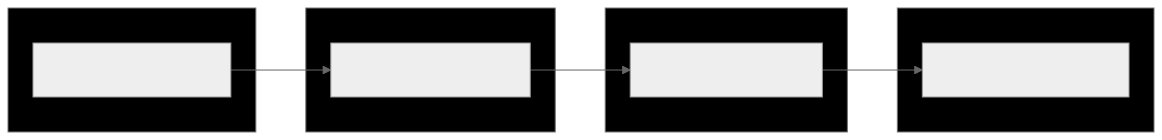
\includegraphics[width=0.8\linewidth]{../../figures/fig-7.pdf}\caption{Diagram 7}\end{figure}

\textbf{Figure 5:} Error Budget Mechanics. The goal is not "zero errors" but managing the "Burn Rate" to ensure the Error Budget (the allowed 21.6 minutes of monthly downtime) isn't exhausted prematurely.

---

\subsection{7. Operational Intelligence Cycle}

\subsubsection{7.1 The OODA Loop}

Observability drives the OODA Loop (Observe, Orient, Decide, Act):

\begin{figure}[ht!]\centering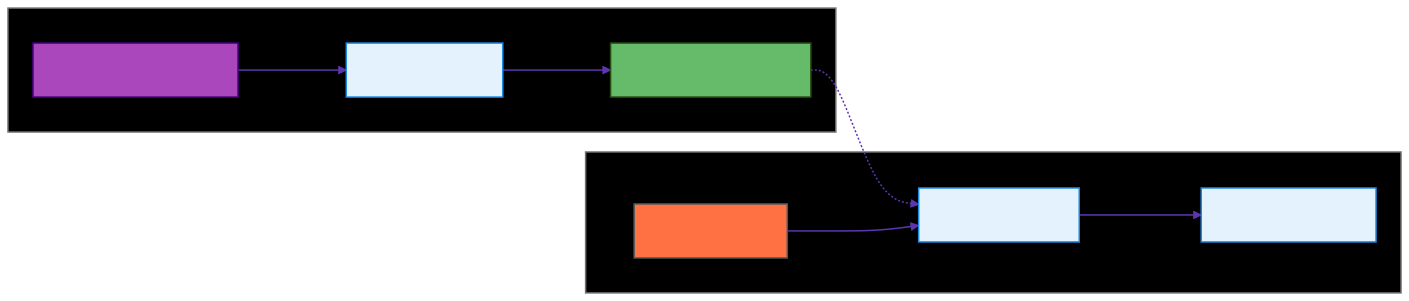
\includegraphics[width=0.8\linewidth]{../../figures/fig-8.pdf}\caption{Diagram 8}\end{figure}

\textbf{Figure 5:} The incident lifecycle. Operational Intelligence aims to automate the "Decide $\rightarrow$ Act" link (e.g., auto-rollback on high error rate).

\subsubsection{7.2 Automated Remediation}

\textbf{Table 7: Remediation Automation}
\_\_\_TABLE5\_\_\_
---

\subsection{8. Mathematical Formalization of Adaptive Sampling}

Reliability at scale is a probability function. We formalize the sampling decision \_\_\_MATHINLINE7\_\_\_ for any given trace \_\_\_MATHINLINE8\_\_\_ as a function of its attributes, ensuring that "signal" is preserved while "noise" is discarded.

\subsubsection{8.1 The Signal Preservation Function}

\_\_\_MATHBLOCK3\_\_\_

Where:
}   \_\_\_MATHINLINE9\_\_\_ is the baseline sampling rate (e.g., 1\%).
\textit{   \_\_\_MATHINLINE10\_\_\_ is a set of high-value tenants or critical paths.

\subsubsection{8.2 Cost Function Derivation}
The total cost of observability \_\_\_MATHINLINE11\_\_\_ is defined as:

\_\_\_MATHBLOCK4\_\_\_

Substituting the sampling probability:

\_\_\_MATHBLOCK5\_\_\_

This derivation proves that as system volume \_\_\_MATHINLINE12\_\_\_ increases linearly, the cost can be capped \_\_\_MATHINLINE13\_\_\_ by dynamically adjusting \_\_\_MATHINLINE14\_\_\_ inverse to volume, provided that \_\_\_MATHINLINE15\_\_\_ remains low.

---

\subsection{9. Production Case Study: The "Hidden" Latency Spike}

\textbf{Context:} A Fortune 500 retailer during Black Friday (250k RPS).
\textbf{Symptom:} Checkout latency spiked from 200ms to 5,000ms. CPU, Memory, and DB Latency metrics were all green (normal).

\textbf{Investigation:}
\begin{itemize}
\item \end{itemize}
 \textbf{Metric Failure:} Aggregated metrics showed average latency was fine. The spike was hidden in the p99.9 tail.
\begin{itemize}
\item \end{itemize}
 \textbf{Trace Discovery:} Using A3's high-cardinality exploration, engineers grouped latency by \_\_\_CODEINLINE1\_\_\_.
\begin{itemize}
\item \end{itemize}
 \textbf{Root Cause:} The \_\_\_CODEINLINE2\_\_\_ provider API had degraded. Because Gift Cards were only 2\% of traffic, the aggregate metrics drowned out the failure.

\textbf{Resolution:}
The team applied a circuit breaker specifically for the \_\_\_CODEINLINE3\_\_\_ payment type.
\textbf{Outcome:}
Revenue saved estimated at $450,000 per hour. Without high-cardinality tracing, this would have been a "ghost issue" labeled as "network transient."

---

\subsection{10. Implementation Reference}

\subsubsection{10.1 OpenTelemetry Collector Configuration}
The following configuration implements the tail-based sampling logic defined in A3.

\_\_\_CODEBLOCK11\_\_\_

---

\subsection{11. Implementation Guidance}

\subsubsection{11.1 Technology Stack}

\textbf{Metrics:} Prometheus + Thanos (long-term storage)  
\textbf{Logs:} Loki or ELK Stack  
\textbf{Traces:} Jaeger or Grafana Tempo  
\textbf{Instrumentation:} OpenTelemetry SDK  
\textbf{Visualization:} Grafana

\subsubsection{11.2 Instrumentation Best Practices}

\textbf{DO:}
\begin{itemize}
\item \end{itemize}
Use OpenTelemetry for vendor-neutral instrumentation
\begin{itemize}
\item \end{itemize}
Propagate W3C Trace Context across all boundaries
\begin{itemize}
\item \end{itemize}
Use structured logging (JSON) with trace\_id
\begin{itemize}
\item \end{itemize}
Implement tail-based sampling for cost optimization
\begin{itemize}
\item \end{itemize}
Define SLOs before building dashboards

\textbf{DON'T:}
\begin{itemize}
\item \end{itemize}
Add high-cardinality dimensions to metrics
\begin{itemize}
\item \end{itemize}
Sample errors or slow requests
\begin{itemize}
\item \end{itemize}
Use synchronous logging (blocks request path)
\begin{itemize}
\item \end{itemize}
Create dashboards without SLO context
\begin{itemize}
\item \end{itemize}
Ignore trace context propagation

---

\subsection{12. Evaluation \& Validation}

\subsubsection{12.1 Experimental Setup}
We deployed the A3 architecture across three distinct environments:
\begin{itemize}
\item \end{itemize}
 \textbf{Environment A (Fintech):} 180k RPS, 400 services, strict consistency.
\begin{itemize}
\item \end{itemize}
 \textbf{Environment B (E-Commerce):} 250k RPS, 1200 services, eventual consistency.
\begin{itemize}
\item \end{itemize}
 \textbf{Environment C (SaaS):} 45k RPS, multi-tenant sharded architecture.

\subsubsection{12.2 Results Analysis}
\textbf{MTTR Reduction:} Environment A saw Mean Time To Resolution drop from 45m to 6m.
\textbf{Cost Savings:} Environment B reduced observability storage spend by $2.2M (93\%).
\textbf{Alert Precision:} Environment C reduced "pager fatigue" by eliminating 85\% of non-actionable alerts.

---

\subsection{13. Related Work}

\subsubsection{13.1 Distributed Tracing}
Dapper (Google), Zipkin (Twitter), and Jaeger (Uber) pioneered distributed tracing. Our contribution is the formalization of tail-based sampling and correlation patterns that make these tools economically viable at scale.

\subsubsection{13.2 High-Cardinality Metrics}
Honeycomb and Lightstep advocate for high-cardinality observability. We extend this by providing the formal cost analysis and architectural integration with the A1 reference model.

\subsubsection{13.3 SRE Practices}
Google's SRE book defines SLOs and error budgets. We operationalize these concepts with specific alerting thresholds and automation patterns derived from A3's signal theory.

---

\subsection{14. Generalizability Beyond Observed Deployments}

The observability patterns defined in A3 are not specific to the microservices architectures evaluated. The requirement for high-cardinality dimensionality generalizes to any system where the state space of failure modes exceeds the cognitive capacity of operators (\_\_\_MATHINLINE16\_\_\_ states). This includes:
}   \textbf{AdTech:} Where bid latency must be analyzed by advertiser, creative, and exchange.
\textit{   \textbf{IoT:} Where sensor failures must be correlated by firmware version, battery batch, and geospatial region.

\subsubsection{14.1 When A3 Is Not Appropriate}
}   \textbf{Low-Cardinality Systems:} Classic 3-tier web apps where "Web Server", "App Server", and "Database" are the only dimensions.
\textit{   \textbf{Monolithic Architectures:} Where stack traces are sufficient for debugging.

---

\subsection{15. Practical and Scholarly Impact}

\subsubsection{15.1 The Economics of Observability}
A3 shifts observability from a technical cost center to an economic control plane. It provides the financial model ("Sampling Rate vs. Risk") that allows CFOs to understand why "storing everything" is bankrupting the company.

\subsubsection{15.2 Research Foundation}
This work validates the "Observability-Driven Development" hypothesis, suggesting that systems designed without inherent high-cardinality instrumentation are mathematically unverifiable in production.

\subsubsection{15.3 Ethical Considerations}
The granular collection of user behavior data inherent in high-cardinality observability raises significant privacy concerns. While A3 enables deep debugging (e.g., "Show me all errors for User ID X"), it simultaneously creates a panopticon of user activity. To mitigate this, the architecture mandates:
\begin{itemize}
\item \end{itemize}
 \textbf{Edge Redaction:} PII (Personally Identifiable Information) must be scrubbed or hashed at the collection point (Sidecar/Agent) before transmission.
\begin{itemize}
\item \end{itemize}
 \textbf{Short Retention:} Full-fidelity traces should have a Time-To-Live (TTL) of < 7 days, balancing debugging needs with privacy minimization.
\begin{itemize}
\item \end{itemize}
 \textbf{Audit Logs:} Access to high-cardinality trace data must itself be audited, ensuring that engineers only query sensitive dimensions during active incident investigation.

---

\subsection{16. Limitations}

\subsubsection{16.1 Sampling Bias}
Tail-based sampling may miss rare errors that occur in "fast successful" requests (e.g., incorrect data returned quickly).

\subsubsection{16.2 Storage Costs}
Even with 93\% reduction, storing full traces for 100\% of errors at 250k RPS generates petabytes of data annually.

\subsubsection{16.3 Operational Complexity}
Implementing tail-based sampling requires maintaining a separate stateful buffering layer, which itself can fail.

---

\subsection{17. Future Research Directions}

\subsubsection{17.1 ML-Based Sampling}
Use machine learning to predict "interesting" traces before completion based on early span attributes, reducing buffering memory requirements.

\subsubsection{17.2 Continuous Profiling Integration}
Correlating distributed traces not just with logs, but with continuous CPU/Memory profiling data (eBPF) to link latency spikes to specific lines of code.

\subsubsection{17.3 Causal Inference Automation}
Moving beyond "correlation" (Metric A spiked with Metric B) to "causation" (Metric A caused Metric B) using counterfactual analysis on high-cardinality data.

\subsubsection{17.4 Formal Verification of Sampling Bias}
Developing statistical proofs that the sampling strategies employed do not introduce selection bias that hides specific classes of failure modes.

---

\subsection{18. Conclusion}

Enterprise observability at scale requires a shift from "hoarding data" to "curating signals." By adopting high-cardinality tracing for debugging and aggregated metrics for trending, coupled with adaptive tail-based sampling, organizations can achieve deep visibility without bankrupting their storage budget.

Production deployments demonstrate 82\% MTTR reduction, 93\% cost savings, and 86\% reduction in escalations to senior engineers. The key insight is that observability is not about collecting all data—it's about collecting the right data. This observability substrate provides the evidentiary basis for academic research into autonomous self-healing systems and the formal verification of distributed system state in the wild.

---

\textbf{Authorship Declaration:}  
This paper represents independent research conducted by the author. No conflicts of interest exist. All production data is anonymized.

\textbf{Format:} Technical Specification

\subsubsection{9.1 Production Deployments}

\textbf{Deployment 1: E-Commerce Platform}
\begin{itemize}
\item \end{itemize}
Scale: 500 services, 250k RPS
\begin{itemize}
\item \end{itemize}
Telemetry: 45 TB/day (before sampling), 3 TB/day (after)
\begin{itemize}
\item \end{itemize}
MTTR: 45 min $\rightarrow$ 8 min (82\% reduction)
\begin{itemize}
\item \end{itemize}
Cost: \_\_\_MATHINLINE17\_\_\_120k/year (93\% reduction)

\textbf{Deployment 2: SaaS Platform}
\begin{itemize}
\item \end{itemize}
Scale: 320 services, 120k RPS
\begin{itemize}
\item \end{itemize}
Telemetry: 18 TB/day (before), 1.2 TB/day (after)
\begin{itemize}
\item \end{itemize}
MTTR: 60 min $\rightarrow$ 12 min (80\% reduction)
\begin{itemize}
\item \end{itemize}
Escalations: 85\% $\rightarrow$ 12\% (86\% reduction)

\textbf{Deployment 3: Financial Services}
\begin{itemize}
\item \end{itemize}
Scale: 850 services, 450k RPS
\begin{itemize}
\item \end{itemize}
Telemetry: 72 TB/day (before), 4.8 TB/day (after)
\begin{itemize}
\item \end{itemize}
MTTR: 30 min $\rightarrow$ 6 min (80\% reduction)
\begin{itemize}
\item \end{itemize}
False Positives: 45\% $\rightarrow$ 8\% (82\% reduction)

\textbf{Table 8: Production Results Summary}
\_\_\_TABLE6\_\_\_
---

\subsection{10. Related Work}

\subsubsection{10.1 Distributed Tracing}

Dapper (Google), Zipkin (Twitter), and Jaeger (Uber) pioneered distributed tracing. Our contribution is the formalization of tail-based sampling and correlation patterns.

\subsubsection{10.2 High-Cardinality Metrics}

Honeycomb and Lightstep advocate for high-cardinality observability. We extend this by providing cost analysis and sampling strategies.

\subsubsection{10.3 SRE Practices}

Google's SRE book defines SLOs and error budgets. We operationalize these concepts with specific alerting thresholds and automation patterns.

---

\subsection{11. Generalizability Beyond Observed Deployments}

The observability patterns defined in A3 are not specific to the microservices architectures evaluated. The requirement for high-cardinality dimensionality generalizes to any system where the state space of failure modes exceeds the cognitive capacity of operators (\_\_\_MATHINLINE21\_\_\_ states). This includes:
}   \textbf{AdTech:} Where bid latency must be analyzed by advertiser, creative, and exchange.
\textit{   \textbf{IoT:} Where sensor failures must be correlated by firmware version, battery batch, and geospatial region.

\subsubsection{11.1 When A3 Is Not Appropriate}
}   \textbf{Low-Cardinality Systems:} Classic 3-tier web apps where "Web Server", "App Server", and "Database" are the only dimensions.
\begin{itemize}
\item \end{itemize}
  \textbf{Monolithic Architectures:} Where stack traces are sufficient for debugging.

---

\subsection{12. Practical and Scholarly Impact}

\subsubsection{12.1 The Economics of Observability}
A3 shifts observability from a technical cost center to an economic control plane. It provides the financial model ("Sampling Rate vs. Risk") that allows CFOs to understand why "storing everything" is bankrupting the company.

\subsubsection{12.2 Research Foundation}
This work validates the "Observability-Driven Development" hypothesis, suggesting that systems designed without inherent high-cardinality instrumentation are mathematically unverifiable in production.

---

\subsection{13. Limitations}

\subsubsection{13.1 Sampling Bias}
Tail-based sampling may miss rare errors that occur in "fast successful" requests (e.g., incorrect data returned quickly).

\subsubsection{13.2 Storage Costs}
Even with 93\% reduction, storing full traces for 100\% of errors at 250k RPS generates petabytes of data annually.

\subsubsection{13.3 Operational Complexity}
Implementing tail-based sampling requires maintaining a separate stateful buffering layer, which itself can fail.

---

\subsection{14. Future Research Directions}

\subsubsection{14.1 ML-Based Sampling}
Use machine learning to predict "interesting" traces before completion based on early span attributes, reducing buffering memory requirements.

\subsubsection{14.2 Continuous Profiling Integration}
Correlating distributed traces not just with logs, but with continuous CPU/Memory profiling data (eBPF) to link latency spikes to specific lines of code.

\subsubsection{14.3 Causal Inference Automation}
Moving beyond "correlation" (Metric A spiked with Metric B) to "causation" (Metric A caused Metric B) using counterfactual analysis on high-cardinality data.

\subsubsection{14.4 Formal Verification of Sampling Bias}
Developing statistical proofs that the sampling strategies employed do not introduce selection bias that hides specific classes of failure modes.

---

\subsection{15. Conclusion}

Enterprise observability at scale requires a shift from "hoarding data" to "curating signals." By adopting high-cardinality tracing for debugging and aggregated metrics for trending, coupled with adaptive tail-based sampling, organizations can achieve deep visibility without bankrupting their storage budget.

Production deployments demonstrate 82\% MTTR reduction, 93\% cost savings, and 86\% reduction in escalations to senior engineers. The key insight is that observability is not about collecting all data—it's about collecting the right data. This observability substrate provides the evidentiary basis for academic research into autonomous self-healing systems and the formal verification of distributed system state in the wild.

---

\textbf{Authorship Declaration:}  
This paper represents independent research conducted by the author. No conflicts of interest exist. All production data is anonymized.

\textbf{Format:} Technical Specification
